\chapterimage{chapter_head_2.pdf} % Chapter heading image
\chapter{Sensation \& Perception}
\minitoc
\newpage


\section{Sensation}\index{Sensation}

What does it mean to sense something? Sensory receptors are specialized neurons that respond to specific types of stimuli. When sensory information is detected by a sensory receptor, sensation has occurred. For example, light that enters the eye causes chemical changes in photoreceptor cells that line the back of the eye. When these cells are stimulated, messages, in the form of action potentials, are relayed to the central nervous system. The conversion from sensory stimulus energy to action potential is known as \gls{transduction}.

You have probably known since elementary school that we have five senses: vision, hearing (audition), smell (olfaction), taste (gustation), and touch (somatosensation). It turns out that this notion of five senses is oversimplified. We also have sensory systems that provide information about balance (the vestibular sense), body position and movement (proprioception and kinesthesia), pain (nociception), and temperature (thermoception).

Each of these sensory systems uses its own sensory receptors for transduction and, based on the description just provided, you might be inclined to think that questions about sensation are thus purely physical and binary in nature.  For example, how intense (i.e., loud) must a sound be in order for it to be sensed? That this is a psychological question may not be immediately obvious, In fact, this is a common misconception about the study of sensation.   .

The sensitivity of a given sensory system to the relevant stimuli can be expressed as an absolute threshold. Absolute threshold refers to the minimum amount of stimulus energy that must be present for the stimulus to be detected 50\% of the time. Another way to think about this is by asking how dim can a light be or how soft can a sound be and still be detected half of the time. The sensitivity of our sensory receptors can be quite amazing. It has been estimated that on a clear night, the most sensitive sensory cells in the back of the eye can detect a candle flame 30 miles away (Okawa \& Sampath, 2007). Under quiet conditions, the hair cells (the receptor cells of the inner ear) can detect the tick of a clock 20 feet away (Galanter, 1962).

It is also possible for us to get messages that are presented below the threshold for conscious awareness—these are called subliminal messages. A stimulus reaches a physiological threshold when it is strong enough to excite sensory receptors and send nerve impulses to the brain: This is an absolute threshold. A message below that threshold is said to be subliminal: We receive it, but we are not consciously aware of it. Over the years there has been a great deal of speculation about the use of subliminal messages in advertising, rock music, and self-help audio programs. Research evidence shows that in laboratory settings, people can process and respond to information outside of awareness. But this does not mean that we obey these messages like zombies; in fact, hidden messages have little effect on behavior outside the laboratory (Kunst-Wilson \& Zajonc, 1980; Rensink, 2004; Nelson, 2008; Radel, Sarrazin, Legrain, \& Gobancé, 2009; Loersch, Durso, \& Petty, 2013).

Absolute thresholds are generally measured under incredibly controlled conditions in situations that are optimal for sensitivity. Sometimes, we are more interested in how much difference in stimuli is required to detect a difference between them. This is known as the just noticeable difference (jnd) or difference threshold. Unlike the absolute threshold, the difference threshold changes depending on the stimulus intensity. As an example, imagine yourself in a very dark movie theater. If an audience member were to receive a text message on her cell phone which caused her screen to light up, chances are that many people would notice the change in illumination in the theater. However, if the same thing happened in a brightly lit arena during a basketball game, very few people would notice. The cell phone brightness does not change, but its ability to be detected as a change in illumination varies dramatically between the two contexts. Ernst Weber proposed this theory of change in difference threshold in the 1830s, and it has become known as Weber’s law: The difference threshold is a constant fraction of the original stimulus, as the example illustrates.


%------------------------------------------------

\section{Perception}\index{Perception}
%\section{Citation}\index{Citation}
This statement requires citation \cite{article_key}; this one is more specific \cite[162]{book_key}.
While our sensory receptors are constantly collecting information from the environment, it is ultimately how we interpret that information that affects how we interact with the world. Perception refers to the way sensory information is organized, interpreted, and consciously experienced. Perception involves both bottom-up and top-down processing. Bottom-up processing refers to the fact that perceptions are built from sensory input. On the other hand, how we interpret those sensations is influenced by our available knowledge, our experiences, and our thoughts. This is called top-down processing.

One way to think of this concept is that sensation is a physical process, whereas perception is psychological. For example, upon walking into a kitchen and smelling the scent of baking cinnamon rolls, the sensation is the scent receptors detecting the odor of cinnamon, but the perception may be ``Mmm, this smells like the bread Grandma used to bake when the family gathered for holidays."

Although our perceptions are built from sensations, not all sensations result in perception. In fact, we often don’t perceive stimuli that remain relatively constant over prolonged periods of time. This is known as sensory adaptation. Imagine entering a classroom with an old analog clock. Upon first entering the room, you can hear the ticking of the clock; as you begin to engage in conversation with classmates or listen to your professor greet the class, you are no longer aware of the ticking. The clock is still ticking, and that information is still affecting sensory receptors of the auditory system. The fact that you no longer perceive the sound demonstrates sensory adaptation and shows that while closely associated, sensation and perception are different.

There is another factor that affects sensation and perception: attention. Attention plays a significant role in determining what is sensed versus what is perceived. Imagine you are at a party full of music, chatter, and laughter. You get involved in an interesting conversation with a friend, and you tune out all the background noise. If someone interrupted you to ask what song had just finished playing, you would probably be unable to answer that question.

\begin{corollary}[Selective Attention]
Click \href{https://www.youtube.com/watch?v=vJG698U2Mvo}{HERE} to see for yourself how inattentional blindness works in a demonstration of selective attention from Simons and Chabris (1999). 
\end{corollary}

One of the most interesting demonstrations of how important attention is in determining our perception of the environment occurred in a famous study conducted by Daniel Simons and Christopher Chabris (1999). In this study, participants watched a video of people dressed in black and white passing basketballs. Participants were asked to count the number of times the team in white passed the ball. During the video, a person dressed in a black gorilla costume walks among the two teams. You would think that someone would notice the gorilla, right? Nearly half of the people who watched the video didn’t notice the gorilla at all, despite the fact that he was clearly visible for nine seconds. Because participants were so focused on the number of times the white team was passing the ball, they completely tuned out other visual information. Failure to notice something that is completely visible because of a lack of attention is called inattentional blindness.

In a similar experiment, researchers tested inattentional blindness by asking participants to observe images moving across a computer screen. They were instructed to focus on either white or black objects, disregarding the other color. When a red cross passed across the screen, about one third of subjects did not notice it (Figure \ref{fig:perception1} (Most, Simons, Scholl, \& Chabris, 2000).

\begin{figure}[ht]
\centering
\includegraphics[scale=1.5]{perception1.jpg}
\caption{Nearly one third of participants in a study did not notice that a red cross passed on the screen because their attention was focused on the black or white figures. (credit: Cory Zanker)}
\label{fig:perception1} % Unique label used for referencing the figure in-text
%\addcontentsline{toc}{figure}{Figure \ref{fig:placeholder}} % Uncomment to add the figure to the table of contents
\end{figure}

Motivation can also affect perception. Have you ever been expecting a really important phone call and, while taking a shower, you think you hear the phone ringing, only to discover that it is not? If so, then you have experienced how motivation to detect a meaningful stimulus can shift our ability to discriminate between a true sensory stimulus and background noise. The ability to identify a stimulus when it is embedded in a distracting background is called signal detection theory. This might also explain why a mother is awakened by a quiet murmur from her baby but not by other sounds that occur while she is asleep. Signal detection theory has practical applications, such as increasing air traffic controller accuracy. Controllers need to be able to detect planes among many signals (blips) that appear on the radar screen and follow those planes as they move through the sky. In fact, the original work of the researcher who developed signal detection theory was focused on improving the sensitivity of air traffic controllers to plane blips (Swets, 1964).

Our perceptions can also be affected by our beliefs, values, prejudices, expectations, and life experiences. As you will see later in this chapter, individuals who are deprived of the experience of binocular vision during critical periods of development have trouble perceiving depth (Fawcett, Wang, \& Birch, 2005). The shared experiences of people within a given cultural context can have pronounced effects on perception. For example, Marshall Segall, Donald Campbell, and Melville Herskovits (1963) published the results of a multinational study in which they demonstrated that individuals from Western cultures were more prone to experience certain types of visual illusions than individuals from non-Western cultures, and vice versa. One such illusion that Westerners were more likely to experience was the M\"{u}ller-Lyer illusion (Figure \ref{fig:mullerlyer}): The lines appear to be different lengths, but they are actually the same length.

\begin{figure}[ht]
\centering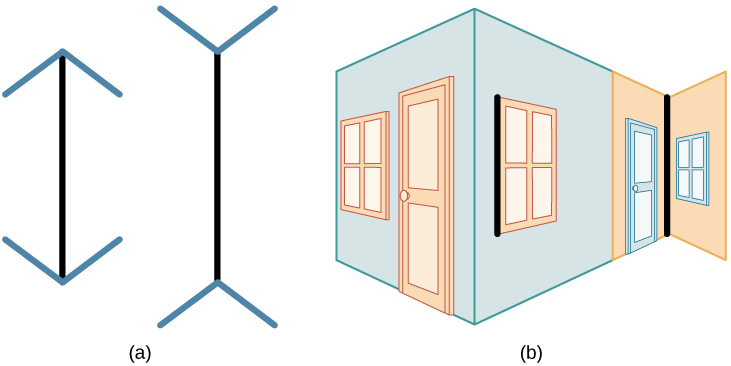
\includegraphics[scale=1]{mullerlyer.jpg}
\caption{ In the M\"{u}ller-Lyer illusion, lines appear to be different lengths although they are identical. (a) Arrows at the ends of lines may make the line on the right appear longer, although the lines are the same length. (b) When applied to a three-dimensional image, the line on the right again may appear longer although both black lines are the same length.}
\label{fig:mullerlyer} % Unique label used for referencing the figure in-text
%\addcontentsline{toc}{figure}{Figure \ref{fig:placeholder}} % Uncomment to add the figure to the table of contents
\end{figure}

These perceptual differences were consistent with differences in the types of environmental features experienced on a regular basis by people in a given cultural context. People in Western cultures, for example, have a perceptual context of buildings with straight lines, what Segall’s study called a carpentered world (Segall et al., 1966). In contrast, people from certain non-Western cultures with an uncarpentered view, such as the Zulu of South Africa, whose villages are made up of round huts arranged in circles, are less susceptible to this illusion (Segall et al., 1999). It is not just vision that is affected by cultural factors. Indeed, research has demonstrated that the ability to identify an odor, and rate its pleasantness and its intensity, varies cross-culturally (Ayabe-Kanamura, Saito, Distel, Martínez-G\'{o}mez, \& Hudson, 1998).

Children described as thrill seekers are more likely to show taste preferences for intense sour flavors (Liem, Westerbeek, Wolterink, Kok, \& de Graaf, 2004), which suggests that basic aspects of personality might affect perception. Furthermore, individuals who hold positive attitudes toward reduced-fat foods are more likely to rate foods labeled as reduced fat as tasting better than people who have less positive attitudes about these products (Aaron, Mela, \& Evans, 1994).
%------------------------------------------------
\newpage